\documentclass{article}

\usepackage[margin=2.5cm]{geometry}

\usepackage[scientific-notation=true, binary-units=true]{siunitx}
\sisetup{per-mode=fraction}%
\sisetup{scientific-notation=false}%
\usepackage{amsmath}
\usepackage{forest}

\usepackage{afterpage}
\usepackage{pdflscape}

\usepackage{tikz}
\usetikzlibrary{shapes,arrows}
\usetikzlibrary{positioning}

\tikzstyle{block} = [rectangle, draw, fill=white!20, 
     text centered, rounded corners, minimum height=3em]
\tikzstyle{blob} = [circle, draw, fill=white!20, 
    text width=2em, text centered, rounded corners, minimum height=2em]
\tikzstyle{cloud} = [draw, ellipse,fill=white!20, node distance=3cm,
    minimum height=2em]
\tikzstyle{arrow} = [thick,->,>=stealth]

\title{SYSC 4502 Assignment 4}
\date{April 7th, 2017}
\author{Jessica Morris \(100882290\)}

\begin{document}

\maketitle

\begin{enumerate}

\item
\begin{enumerate}

\item The output will be 00000101 repeated eight times.

\item The output will be 00000101 repeated seven times, ended with 10000101.

\item For (a), the output will be 10100000 repeated eight times. For (b), the output will be 10100001 followed by 
10100000 repeated seven times.

\end{enumerate}

\item
\begin{enumerate}

\item $ n = p \times q = 5 \times 11 = 55 $, $ z = (p-1)(q-1) = 4 \times 10 = 40 $

\item $ e = 3 $ is acceptable because it is less than $n$, and has no common factors with $z$.

\item $$ de = 1(\text{mod } z) $$
$$ 3d = 1(\text{mod } 40) $$
$$ d = \frac{1(\text{mod } 40)}{3} $$
The nearest integer that gives $ x = 1(\text{mod } 40) $ and is divisible by 3 is 81. Therefore:
$$ d = \frac{81}{3} $$
$$ d = 27 $$

\item For $ m = 8 $, the ciphertext $c$ is:
$$ c = m^e \text{mod } n $$
$$ c = 8^3 \text{mod } 55 $$
$$ c = 512 \text{mod } 55 $$
$$ c = 17 $$

\end{enumerate}

\item Bob's steps to decode the package from Alice:

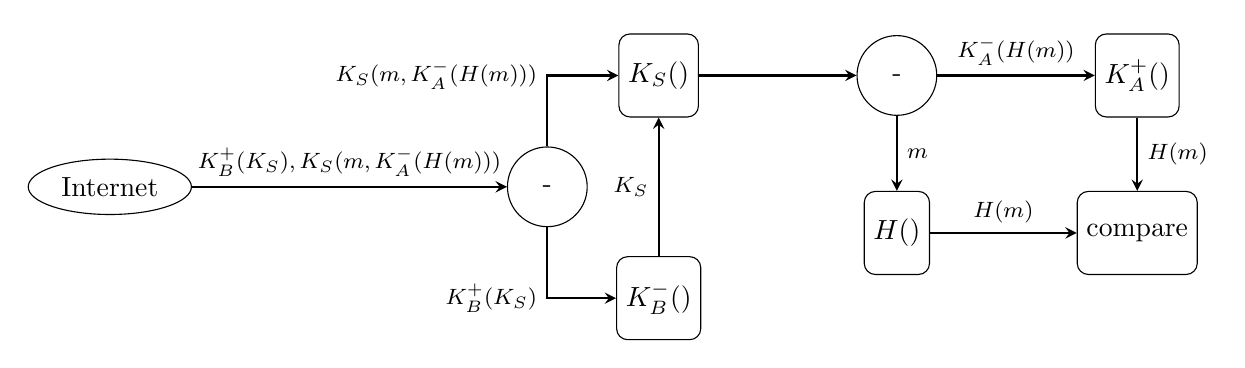
\begin{tikzpicture}[node distance = 2cm, auto]
    % Place nodes
    \node [cloud] (internet) {Internet};
    \node [blob, right=4cm of internet] (sub1) {-};
    \node [block, above right of=sub1] (ks) {$K_S()$};
    \node [block, below right of=sub1] (kb) {$K_B^-()$};
    \node [blob, right=2cm of ks] (sub2) {-};
    \node [block, below of=sub2] (h) {$H()$};
    \node [block, right=2cm of sub2] (ka) {$K_A^+()$};
    \node [block, below of=ka] (compare) {compare};
    
    % Draw edges
    \draw [arrow] (internet) -- node {\footnotesize $K_B^+(K_S),K_S(m,K_A^-(H(m)))$} (sub1);
    \draw [arrow] (sub1) |- node[anchor=east] {\footnotesize $K_S(m,K_A^-(H(m)))$} (ks);
    \draw [arrow] (sub1) |- node[anchor=east] {\footnotesize $K_B^+(K_S)$} (kb);
    \draw [arrow] (kb) -- node {\footnotesize $K_S$} (ks);
    \draw [arrow] (ks) -- (sub2);
    \draw [arrow] (sub2) -- node {\footnotesize $m$} (h);
    \draw [arrow] (sub2) -- node {\footnotesize $K_A^-(H(m))$} (ka);
    \draw [arrow] (h) -- node {\footnotesize $H(m)$} (compare);
    \draw [arrow] (ka) -- node {\footnotesize $H(m)$} (compare);
\end{tikzpicture}

\item
\begin{enumerate}

\item The three fields are (ICV = 1010 pre-encryption):

\begin{tabular}{|c|c|}
    \hline
    IV & 11 \\ \hline
    message & 01011010 \\ \hline
    ICV & 0010 \\ \hline
\end{tabular}

\item Receiver has key = 1010. Since the IV (11) is unencrypted at the beginning of the packet, the receiver uses the 
same keystream to decrypt the packet. XOR'ing the received message + ICV with the keystream results in:
$$ 010110100010 \oplus 111110101000 = 101000001010 $$
The first eight bits give $m = 10100000$ and the last four bits give $ICV=1010$.

\item If Trudy flips the first ICV bit, then she must also flip either the first or the fifth bit of the 
message.

\item The part (a) WEP packet with the first message bit flipped and the first ICV bit flipped is $110110101010$. 
XOR'ing with the 101011 keystream gives:
$$ 1101 1010 1010 \oplus 1111 1010 1000 = 0010 0000 0010 $$

This gives $m=0010 0000$ and $ICV=0010$. The receiver computes the ICV for $m$ to be $0010 \oplus 0000 = 0010$, 
so the ICV check passes.

Alternately, with the fifth message bit flipped, the receiver receives:
$$ 0101 0010 1010 \oplus 111110101000 = 101010000010 $$
This gives $m=1010 1000$ and $ICV=0010$. The receiver computs the ICV for $m$ to be $1010 \oplus 1000 = 0010$, so the 
ICV check passes.

\end{enumerate}


\item Grid-of-Tries: 


    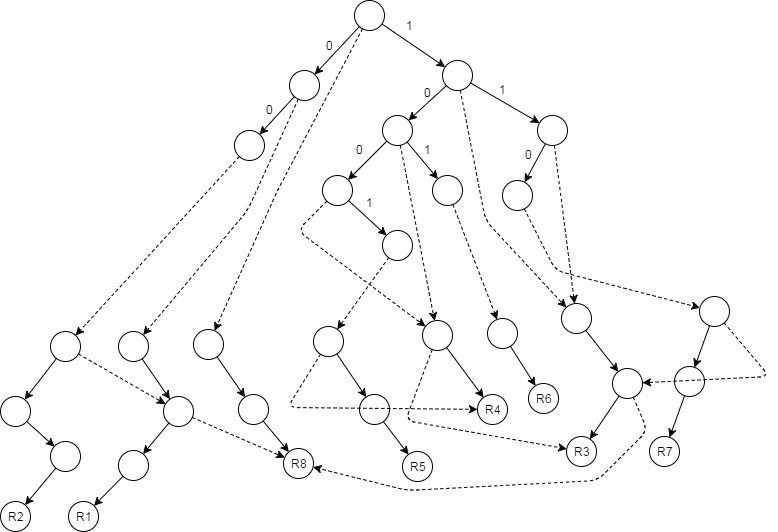
\includegraphics[width=\textwidth]{assignment4_gridoftries}


\item The flow table is as follows:

\begin{tabular}{|c|c|c|c|}
    \hline
    Source IP & In Port & Dest IP & Action \\ \hline
    10.3.0.* & 1 & 10.1.0.* & Output port 2 \\ \hline
    10.1.0.* & 2 & 10.3.0.* & Output port 1 \\ \hline
    * & 1 & 10.2.0.3 & Output port 3 \\ \hline
    * & 1 & 10.2.0.4 & Output port 4 \\ \hline
    * & 2 & 10.2.0.3 & Output port 3 \\ \hline
    * & 2 & 10.2.0.4 & Output port 4 \\ \hline
    10.2.0.3 & * & 10.2.0.4 & Output port 4 \\ \hline
    10.2.0.4 & * & 10.2.0.3 & Output port 3 \\ \hline
\end{tabular}

\end{enumerate}
\end{document}
